\documentclass[letterpaper, 11pt]{article}
\usepackage[margin=1in]{geometry}
\usepackage{graphicx}
\usepackage{amssymb}
\usepackage{epstopdf}
\usepackage{url}
\usepackage{hyperref}
\usepackage{graphicx}
\usepackage{amsmath}

\newcommand{\ft}{$\vec{f}^t$}

\title{CS175 - Assignment 2 \\Playing with Frames (on paper)}

\begin{document}
\noindent \textbf{(4.1)} \\ 
The first transformation considers left to right. So, \ft is rotated, and that rotated frame is translated around its new $x$-axis. 

\medskip
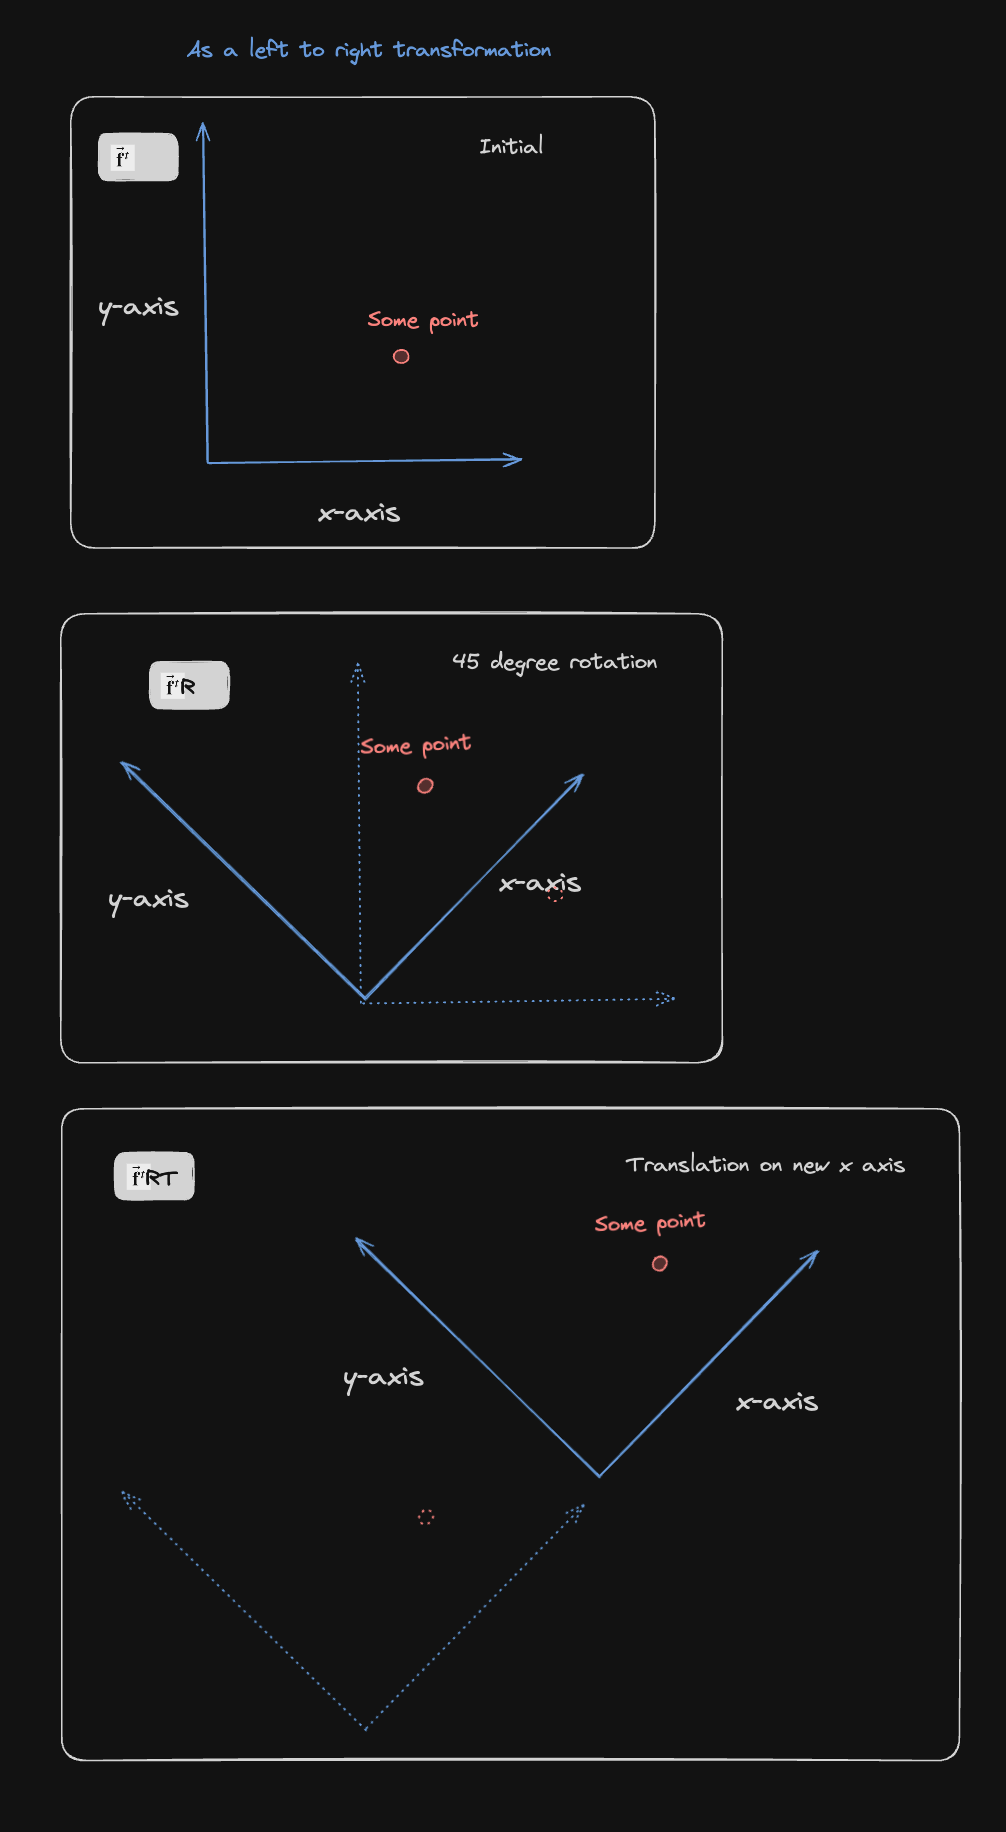
\includegraphics[scale=0.6]{./pics/q1_ltr.png}

\newpage
\medskip
\noindent The second transformation considers right to left. Here, \ft is translated along its original $x$-axis. But then it's rotated around the original frame's origin. This produces the same result. 

\medskip
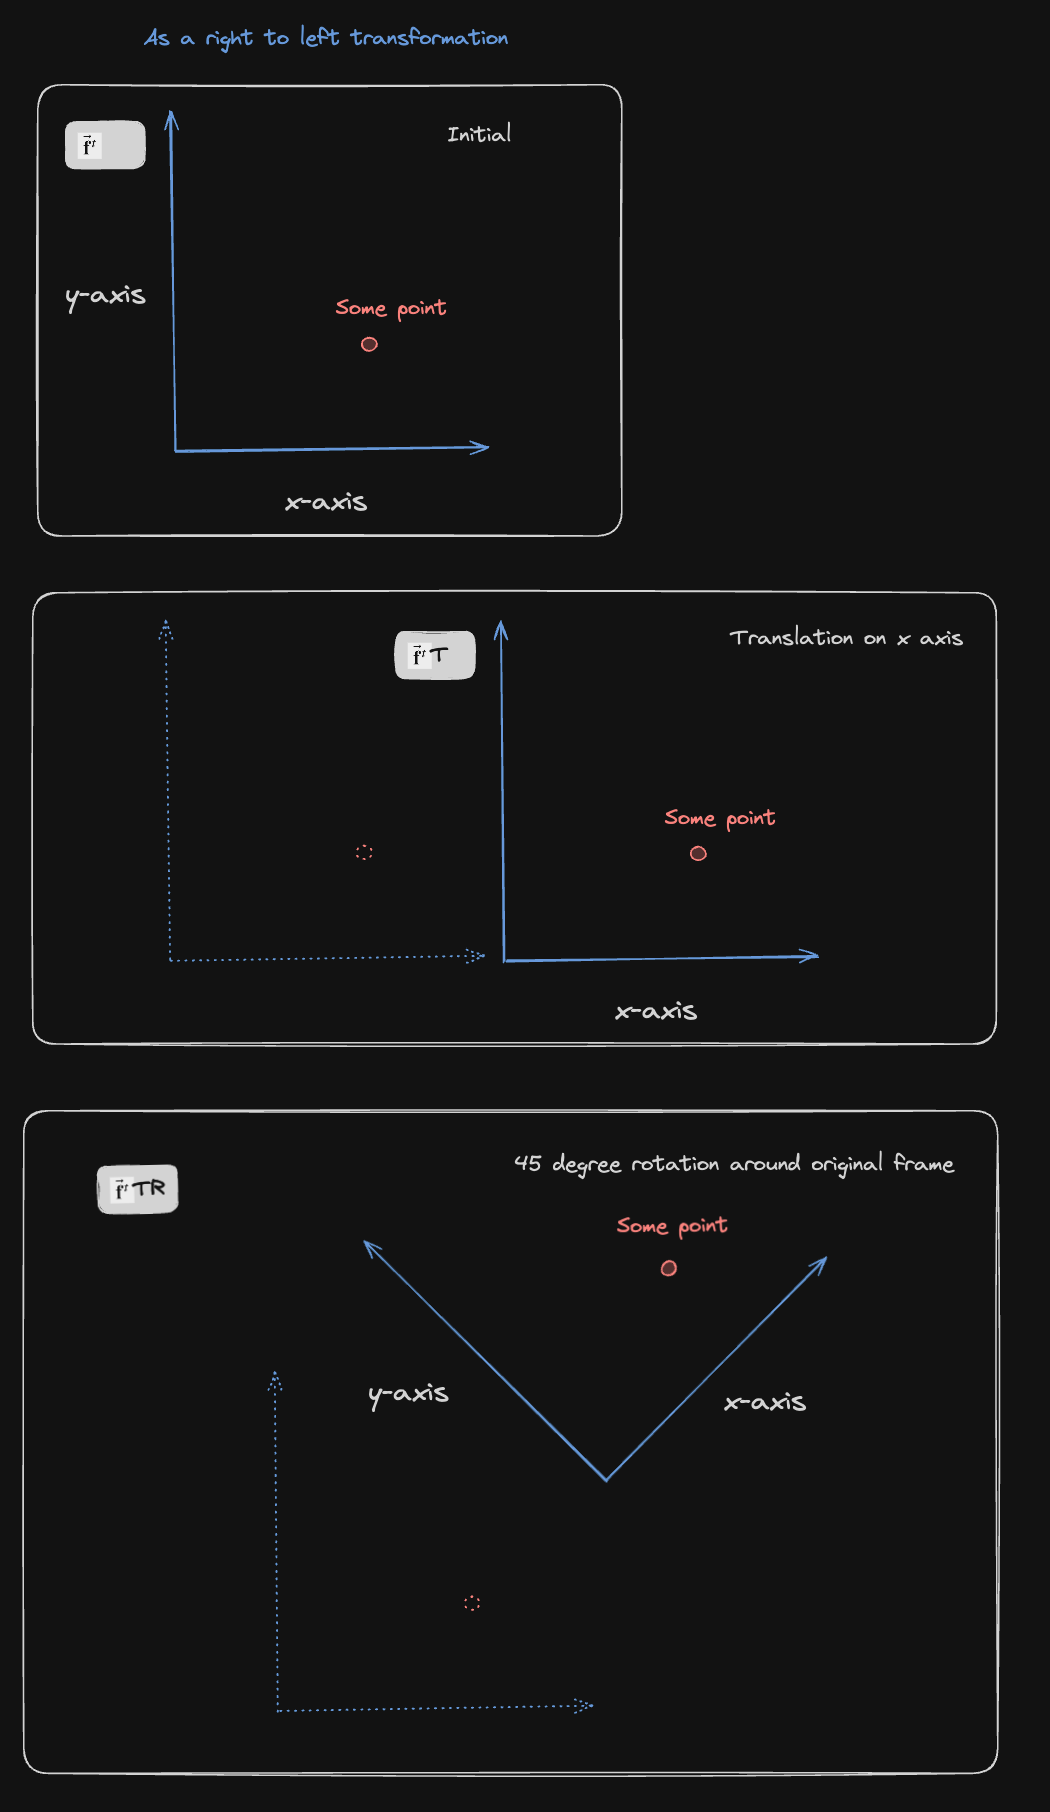
\includegraphics[scale=0.6]{./pics/q1_rtl.png}

\newpage 
\noindent \textbf{(4.2)} \\ 
The origin is now $2$ \ft units from where it started. Once $S$ is applied uniformly to \ft, one unit of \ft$S$ is now two units of \ft. Thus, translating \ft$S$ by one unit translates by two units of \ft. Because there is no rotation, this is the only movement of the origin. The picture below represents this. A right to left perspective yields the same result. An initial translation makes \ft$T$ one unit away from the origin of \ft. Scaling that by $2$ makes \ft$ST$ now $2$ units away from the origin of \ft.

\medskip
\noindent 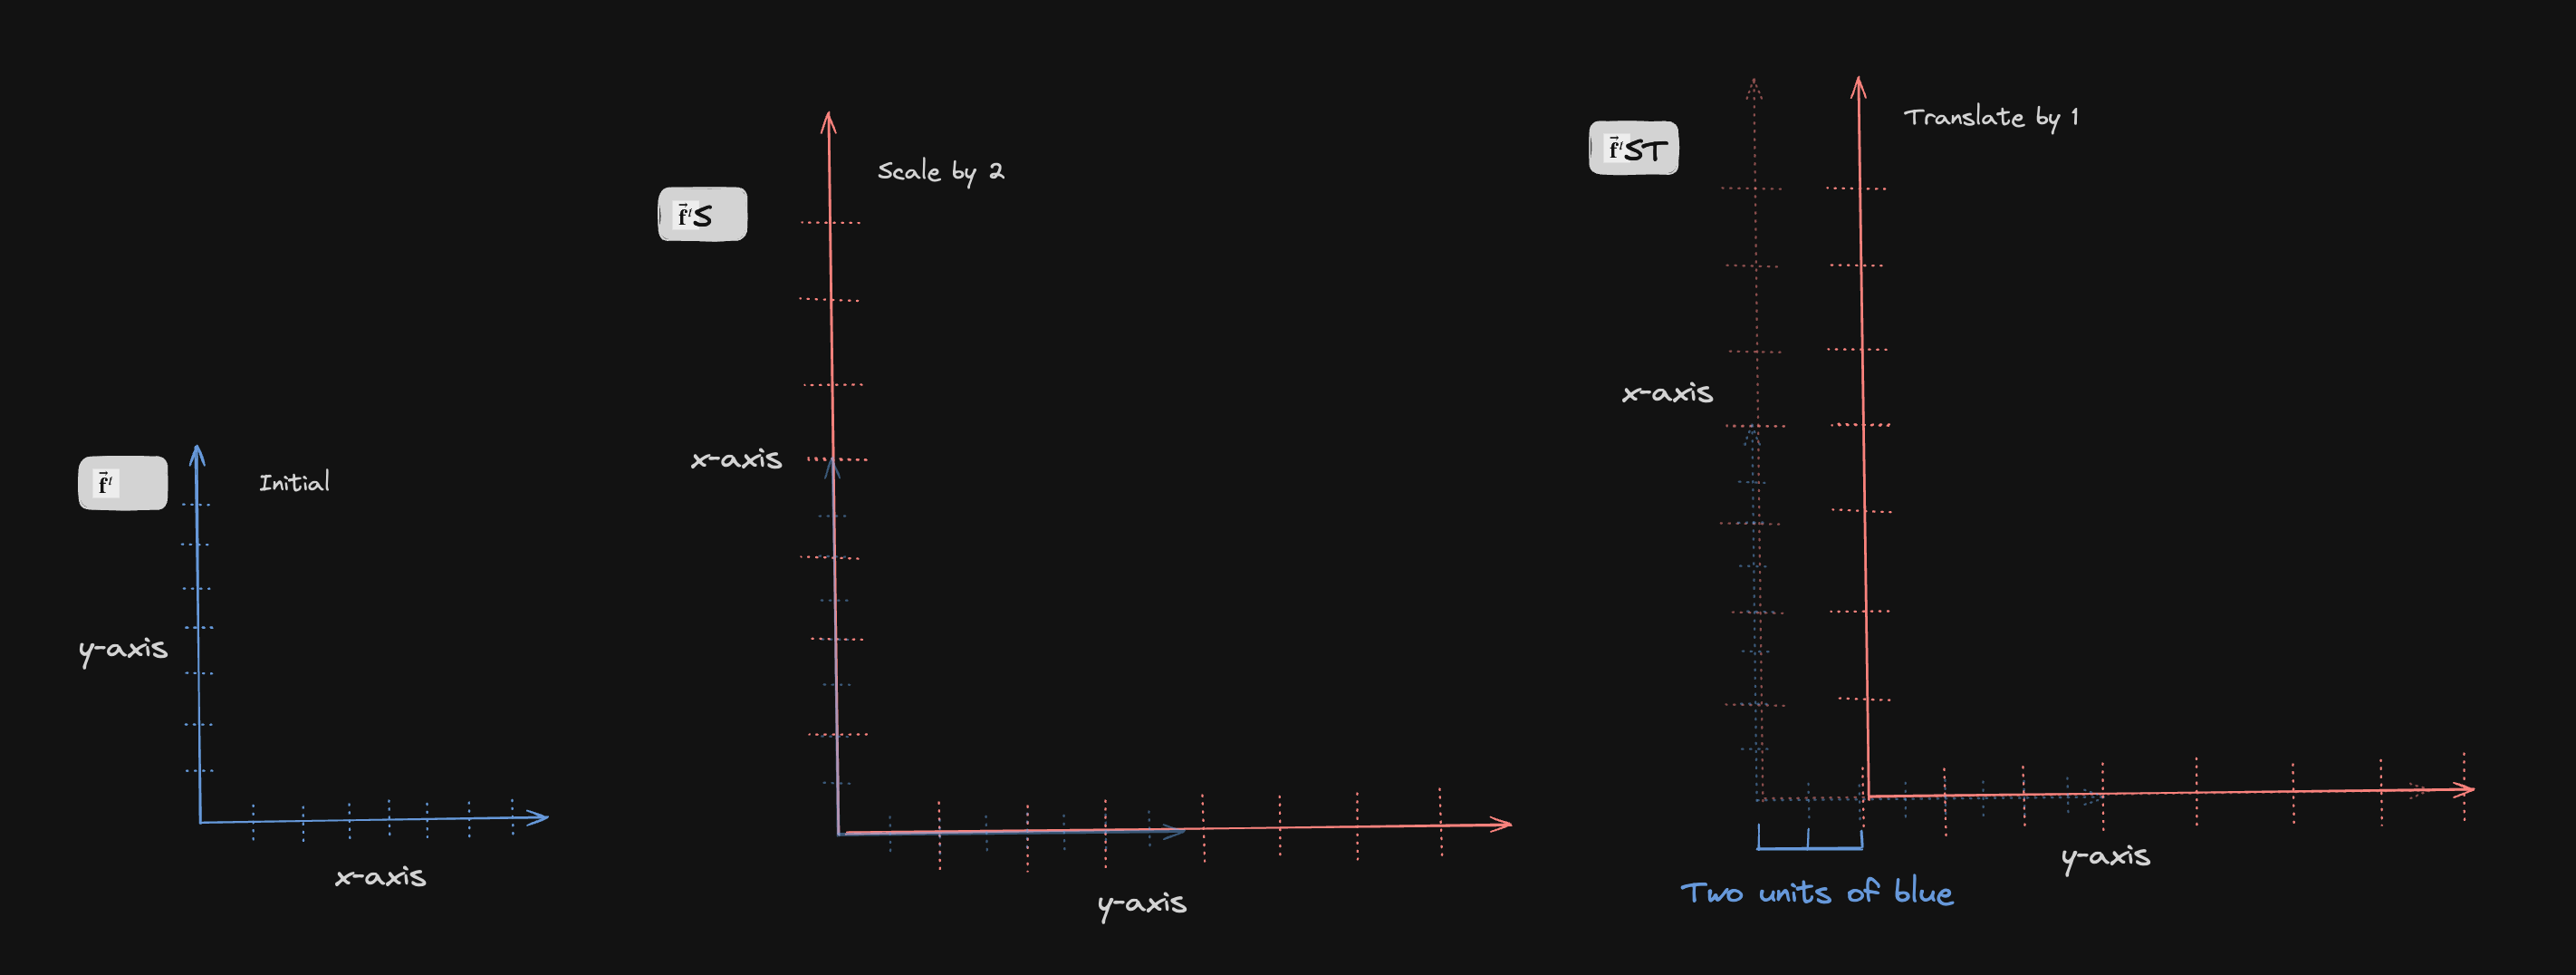
\includegraphics[scale=0.3]{./pics/q2.png}

\newpage
\noindent \textbf{(4.3)} \\
$\vec{b}^t = \vec{a}^t TR$: \\
Because $\vec{a}^t$ is a frame, it's possible to apply an affine translation. From $\vec{a}^t$, the transformation moves by $d_1$ in a positive $x$ direction and by $d_2$ in a positive $y$ direction. Encoding this into an affine matrix $T$ yields the following:

$$T = \begin{bmatrix}
  1 & 0 & 0 & d_1 \\
  0 & 1 & 0 & d_2 \\ 
  0 & 0 & 1 & 0 \\ 
  0 & 0 & 0 & 1
\end{bmatrix}$$

Assert from the appearance of the drawing that $d_3$ is parallel to the $x$-axis of $\vec{b}^t$. Thus, $\theta$ is the degree of rotation in $\vec{b}^t$. This yields an affine rotation matrix $R$ defined like this:

$$R = \begin{bmatrix}
  \cos \theta & - \sin \theta & 0 & 0 \\ 
  \sin \theta & \cos \theta & 0 & 0 \\ 
  0 & 0 & 1 & 0 \\ 
  0 & 0 & 0 & 1 \\
\end{bmatrix}$$

\medskip
\noindent $\vec{b}^t = \vec{a}^t RT$: \\
Again, $\vec{b}^t$ is rotated by $\theta$ degrees, so the rotation matrix $R$ is the same:

$$R = \begin{bmatrix}
  \cos \theta & - \sin \theta & 0 & 0 \\ 
  \sin \theta & \cos \theta & 0 & 0 \\ 
  0 & 0 & 1 & 0 \\ 
  0 & 0 & 0 & 1 \\
\end{bmatrix}$$

Now, the line marked $d_3$ is along the $x$ axis, and the line marked $d_4$ is along the $y$ axis. So, $T$ is the affine matrix with those $x$ and $y$ transformations:

$$T = \begin{bmatrix}
  1 & 0 & 0 & d_3 \\
  0 & 1 & 0 & d_4 \\ 
  0 & 0 & 1 & 0 \\ 
  0 & 0 & 0 & 1
\end{bmatrix}$$

\newpage
\noindent \textbf{(4.4)} \\

\end{document}
